\documentclass{article}
\usepackage{graphicx}
\usepackage{float}
% Lydia

\begin{document}

\subsection{Module Requirements: Module LCD}
%The operational scenarios considered place certain requirements on the something system, and on the modules that comprise it.
This section looks at the hardware interfacing of the LCD in both setting it up for output and writing strings to it. Most sections will consist of a 'Hardware' subsection to give detail of the relevant low level hardware interfacing that occurs through software and hardware, followed by 'Writing', which concerns the higher level software that is involved with creating the user output on the LCD, and will make extensive reference to the LCD\textunderscore disp(x,y) function.

LCD\textunderscore disp(x,y) is a Menu mode function written that takes in the current status (namely menu\textunderscore ref\textunderscore 1 and menu\textunderscore ref\textunderscore 2) and prints an appropriate message to the LCD.

\subsubsection{Reference Document}
Much of the initialisation process is informed by these external sources and libraries:
\begin{itemize}
	\item 'LCD Initialization' Donald Weiman 2012, Alfred State.
	\item 'Interfacing LCD with PIC Microcontroller', Ligo George 2014, ElectroSome.
\end{itemize}

The main goal of this module is the appropriate implementation of the LCD with the system and determining how to achieve LCD functionality given the existing platform of information and the hardware we are given.
\subsubsection{Functional Requirements}
The LCD should gives immediate feedback and information to user of current status of system that is relevant to the context of operation. It does so with little latency and maximum clarity and understandability. In the interest of saving pins, the system uses the LCD in 4-bit mode.

\paragraph{Inputs}
%Describe each external input, including signal encoding and timing, message encoding and timing, protocols, file formats, protection against input errors, etc, as relevant.

The LCD hardware consists of 14-inputs given as follows:
\begin{itemize}
	\item 1 - Ground
	\item 2 - Vcc
	\item 3 - Contrast - Connected to output of 10KOhm potentiometer connected to Vcc
	\item 4 - RS Register Select - 0 for LCD instruction; 1 for data read/write; PORTDbits.RD2
	\item 5 - RW Read/Write - Always set to ground as we never read (0 = Write)
	\item 6 - Enable; PORTDbits.RD3
	\item 7-10 - Data bits 0-3; unused in 4-bit mode
	\item 11-14 - Data bits 4-7; Connected to PORTDbits.RD4-7
\end{itemize}
\begin{figure}[H]
		
	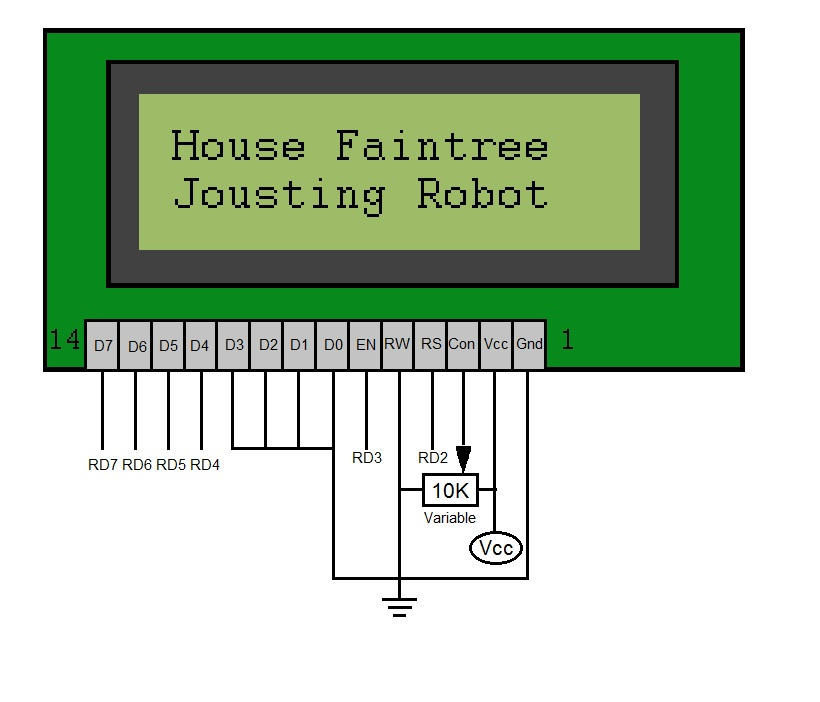
\includegraphics[scale=0.45]{LCD.jpg}
	\centering
	\caption{LCD inputs}
\end{figure}
	These hardware inputs are interfaced by software commands and data through Port D by functions such as LCD\textunderscore init and writing functions.
	The main function that uses the LCD to display a message, LCD\textunderscore write\textunderscore string, takes in a string, while the function LCD\textunderscore disp (which utilises LCD\textunderscore write\textunderscore string)takes in two arguments relating to the status of the commander, menu\textunderscore ref\textunderscore 1 and menu\textunderscore ref\textunderscore 2. 

\paragraph{Process and Output}
%Describe the internal signal transformations and/or computer processing functionality required within the module, required performance limits, and error tolerances as appropriate.

The LCD takes two forms of signals, Commands and Data. Commands are instructions to the LCD that do tasks such as Clear Display, Reset, and Set Cursor and are defined by a 0 value to RS, and nibbles written to RD4-RD7 corresponding to individual commands. Data inputs are read as characters to be written to the LCD and are defined by a 1 value to RS and corresponding nibble to RD4-RD7. EN in both cases is toggled on and off for the LCD to capture the input.\\

Before sending data to the LCD, there is some level of parsing done through LCD\textunderscore disp. Through menu\textunderscore ref\textunderscore 1 it determines the current run-time mode and writes it to the first line. Through menu\textunderscore ref\textunderscore 2, it determines the submenu and displays it in an appropriate manner on the second line:
\begin{itemize}
	\item If a submenu is to be displayed, it is displayed with the label of what it is and its current value. For example, the second line will appear as \texttt{Submenu:Value}
	\item The submenu label string is stored in an array of strings in \texttt{stringtab[ ]} and the respective value is stored in an array of values in \texttt{values[ ]}
	\item Max Speed, Yaw Rate and similar are displayed as percentages; this was determined to be the most intuitive way of presenting this data to users
	\item IR Samples/Estimate, IR Sample Rate and similar are displayed as integers or actual values
	\item No value is displayed on the second line when in the Menu Mode of Assisted and Auto, as per specifications
\end{itemize}


\paragraph{Timing}
%Any required timing or latency specifications that must be met.
For proper initialisation of the LCD, specific delays must be implemented with each initialisation command. This is covered in greater detail in the \underline{Conceptual Design}.

Post Initialisation, the LCD should have no noticeable latency that is attributed to computing latency, nor any timing requirements for basic functionality.


\subsubsection{Non-Function (Quality of Service) Requirements}
LCD in being the main source of data and feedback to the user in implementing desired behaviour should behave in a manner that is comfortable for use.
\paragraph{Performance}
The LCD was determined to only need to be updated (which is a process that requires a clear and then a write) when a variable has actually changed. Initial tests found that constant updating created flickering. Current means of updating LCD results only in a subtle blanking before a new write; again only occurring if a variable were to change.

\paragraph{Design Constraints}
Care should be (and was) exercised when moving software between different processors with different internal clocks. As will be outlined, the function of the LCD depends heavily on correct initialisation which in turn depends heavily on correct settings for delays between commands. Neglecting this will most likely lead to non-function in migration.


\subsection{Conceptual Design: LCD}
%Now, for each module, give the outline of how it will work. In this section it is appropriate to present \\
%•	The rationale for the design decisions that were made – why things were designed the way they were\\
%•	block diagrams,\\
%•	mathematical models and algorithms,\\
%•	data flow diagrams\\
%•	state-transition diagrams\\
%•	listings of input and output formats\\
%•	listings of message and data formats\\
%•	responses to identifiable error conditions\\
%•	responses to identifiable failure conditions\\
%as appropriate for each module.

\subsubsection{Assumptions Made}
The necessary initialisation sequence was based largely off a pre-existing methodology of initialising the LCD; data sheet provides little information of subtle startup commands necessary for initialisation. This is shown in the following flow diagram and is accomplished through LCD\textunderscore init( ).


\begin{figure}[H]
	\vspace*{-2cm}
	\centerline{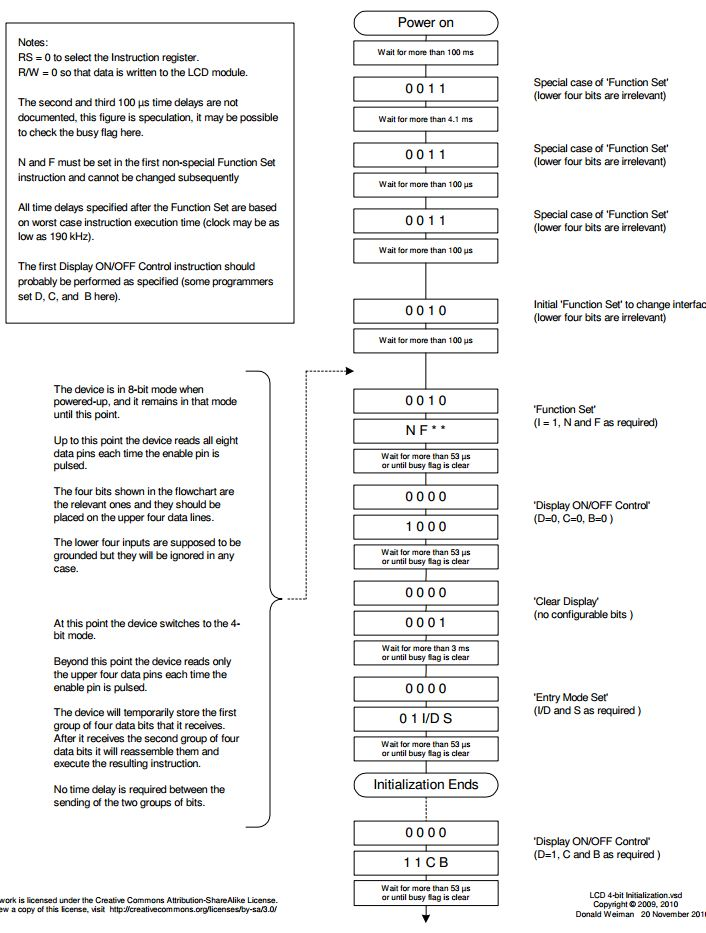
\includegraphics[scale=0.8]{LCDinit.jpg}}
	\centering
	\caption{LCD init data flow}
\end{figure}

\subsubsection{Minor LCD command functions}
\paragraph{\texttt{LCD\textunderscore Port(char data)}} This function was the explicit means of setting the data pins given a char input. It takes the least significant bits and moves and sets the MSBs of the data bits on LCD (as the LSBs are grounded for 4-bit functionality).
\paragraph{\texttt{LCD\textunderscore Cmd(char a)}} This function sends commands by setting RS to 0 for LCD to anticipate a command, use \texttt{LCD\textunderscore Port} to set data bits, EN to 1 to capture command, delaying momentarily, before toggling EN off again.
\paragraph{\texttt{LCD\textunderscore Clear(void)}}
Simply uses \texttt{LCD\textunderscore Cmd} to clear LCD with the clear command (0 then 1).
\paragraph{\texttt{LCD\textunderscore Set\textunderscore Cursor(char row, char col)}} This function takes in two arguments, row and col and sets the cursor position. As their names may suggest, row determines row or line the cursor is moved to and col determines the column. After parsing arguments, function sends command to LCD.

\subsubsection{LCD writing functions}


\end{document}